\chapter{Second Order Differential Equations}
In this brief chapter we will transition back to our discussion of differential equations.
In Chapter 1 we discussed first order linear and nonlinear differential equations and in
this chapter we will discuss second order linear differential equations.  Second order
differential equations arise very naturally from Newton's second law, $ma = \sum F$, since
acceleration is the second derivative of position.  Second order differential equations
also arise naturally in circuit analysis and many other physics-based contexts.  Our
primary focus here will be on mechanical vibrations since that is likely a familar physics
context for most students.

\section{Intro to Second Order Differential Equations}

\begin{problem}
    A branch sways back and forth with position $f(t)$.  Studying its motion you find that
    its acceleration is proportional to its position, so that when it is 8 cm to the
    right, it will accelerate to the left at a rate of 2 cm/s$^2$.  Which differential
    equation describes the motion of the branch?

\begin{enumerate}
    \item[(a)] $\frac{d^2 f}{dt^2} = 8f$
    \item[(b)] $\frac{d^2 f}{dt^2} = -4f$
    \item[(c)] $\frac{d^2 f}{dt^2} = -2$
    \item[(d)] $\frac{d^2 f}{dt^2} = \frac{f}{4}$
    \item[(e)] $\frac{d^2 f}{dt^2} = -\frac{f}{4}$
\end{enumerate}
\end{problem}
% \begin{problem}
%     \begin{itemize}
%             \input{ClickerQuestions/DEQ.00.09.010}
%     \end{itemize}
% \end{problem}
\solution{e}


\begin{problem}
    Which of the following is not a solution of $y'' + ay = 0$ for some value of $a$?

\begin{enumerate}
    \item[(a)] $y = 4 \sin 2 t$
    \item[(b)] $y = 8 \cos 3 t$
    \item[(c)] $y = 2 e^{2t}$
    \item[(d)] all are solutions
\end{enumerate}
\end{problem}
% \begin{problem}
%     \begin{itemize}
%             \input{ClickerQuestions/DEQ.00.09.060}
%     \end{itemize}
% \end{problem}
\solution{d}


\begin{problem}
    The motion of a mass on a spring follows the equation $m x'' = -k x$ where the
    displacement of the mass is given by $x(t)$.  Which of the following would result in
    the highest frequency motion?
\begin{enumerate}
    \item[(a)] $k = 6$, $m=2$
    \item[(b)] $k=4$, $m=4$
    \item[(c)] $k=2$, $m=6$
    \item[(d)] $k = 8$, $m = 6$
    \item[(e)] All frequencies are equal
\end{enumerate}
\end{problem}
% \begin{problem}
%     \begin{itemize}
%             \input{ClickerQuestions/DEQ.00.09.080}
%     \end{itemize}
% \end{problem}
\solution{d}


\begin{problem}
    Which of the following is not a solution of $\frac{d^2 y}{dt^2} = - a y$ for some
    positive value of $a$?
\begin{enumerate}
    \item[(a)] $y = 2 \sin 6t$
    \item[(b)] $y = 4 \cos 5t$
    \item[(c)] $y = 3 \sin 2t + 8 \cos 2t$
    \item[(d)] $y = 2 \sin 3t + 2 \cos 5t$
\end{enumerate}
\end{problem}
% \begin{problem}
%     \begin{itemize}
%             \input{ClickerQuestions/DEQ.00.09.090}
%     \end{itemize}
% \end{problem}
\solution{d}


\begin{problem}
    What function solves the equation $y'' + 10 y =0$?
\begin{enumerate}
    \item[(a)] $y = 10 \sin 10 t$
    \item[(b)] $y = 60 \cos \sqrt{10} t$
    \item[(c)] $y = \sqrt{10} e^{-10 t}$
    \item[(d)] $y = 20 e^{\sqrt{10 t}}$
    \item[(e)] More than one of the above
\end{enumerate}
\end{problem}
% \begin{problem}
%     \begin{itemize}
%             \input{ClickerQuestions/DEQ.00.09.120}
%     \end{itemize}
% \end{problem}
\solution{b}

\begin{technique}[Solving Second Order Linear ODEs]\label{tech:second_order_ode}
    To solve $a y'' + by' + c y = 0$:
    \begin{itemize}
        \item Assume that $y(t) = e^{rt}$
        \item Write the associated characteristic polynomial and use it to find $r$
        \item Write the solution as a linear combination of the linearly independent
            eigenfunctions.  Use the initial conditions to find the constants in the
            linear combination.
        \item Remember to use Euler's Formula if $r$ happens to be complex: 
            \[ e^{i\theta} =\cos(\theta) + i\sin(\theta) \]
    \end{itemize}
\end{technique}


It is worth it here to take a side step and discuss Euler's formula in more detail.  To
understand the roots of Euler's formula we first need to recall the definition of a Taylor
series.
\begin{definition}[Taylor Series]
    Let $f(x)$ be an infinitely differentiable function at a real number $x=a$.  The {\bf
    Taylor Series} of $f(x)$ at $x=a$ is
    \[ f(x) = f(a) + \frac{f'(a)}{1!}(x-a)^1 + \frac{f''(a)}{2!}(x-a)^2
        +\frac{f'''(a)}{3!}(x-a)^3 +\frac{f^{(4)}(a)}{4!}(x-a)^4 + \cdots \]
    The number ``$a$'' is called the center of the Taylor series and if $a=0$ then the
    series is sometimes called a MacLaurin series.
\end{definition}

The Taylor series is a useful tool for approximating functions with simple polynomials.
In fact, every time you use the sine, cosine, and logarithm buttons on your calculator you
are actually just evaluating their Taylor series approximations; your calculator has no
idea what the sine function really is.  

\begin{example}
    Find the Taylor series expansions for the functions $e^x$, $\sin(x)$, and $\cos(x)$
    centered at $a=0$.
    \\{\bf Solution:} 
    We leave it to the reader to take all of the requisite derivatives to verify the
    following.
    \begin{flalign*}
        e^x &= 1 + x + \frac{x^2}{2} + \frac{x^3}{3!} + \frac{x^4}{4!} + \cdots \\
        \sin(x) &= x - \frac{x^3}{3!} + \frac{x^5}{5!} - \frac{x^7}{7!} + \cdots \\
        \cos(x) &= 1 - \frac{x^2}{2!} + \frac{x^4}{4!} - \frac{x^6}{6!} + \cdots
    \end{flalign*}
\end{example}


Now we have all of the tools necessary to verify Euler's formula.  
\begin{problem}
    We would like to verify Euler's formula
    \[ e^{i\theta} = \cos(\theta) + i\sin(\theta). \]
    \begin{enumerate}
        \item[(a)] In the Taylor series for $e^x$ replace the $x$ with $i\theta$.
            \solution{
                \[ e^{i\theta} = 1 + (i\theta) + \frac{(i\theta)^2}{2} +
                    \frac{(i\theta)^3}{3!} + \frac{(i\theta)^4}{4!} +
                    \frac{(i\theta)^5}{5!} + \frac{(i\theta)^6}{6!} +
                    \frac{(i\theta)^7}{7!} \cdots \]
            }
        \item[(b)] Recall that since $i=\sqrt{-1}$ we have
            \[ i^1 = -1, \quad i^3 = -i, \quad i^4 = 1 \]
            and successive powers of $i$ repeat this pattern: $i, -1, -i, 1, i, -1, -i, 1,
            \ldots$.  Simplify each of the powers in your answer to part (a).
            \solution{
                \[ e^{i\theta} = 1 + i\theta - \frac{\theta^2}{2} -
                    i\frac{\theta^3}{3!} + \frac{\theta^4}{4!} + 
                    i\frac{\theta^5}{5!} - \frac{\theta^6}{6!} -
                    i\frac{\theta^7}{7!} \cdots \]
            }
        \item[(c)] Rearrange your answer in part (c) to gather the real terms together and
            the imaginary terms together.
            \solution{
                \[ e^{i\theta} = \left( 1 + - \frac{\theta^2}{2} + \frac{\theta^4}{4!}-
                    \frac{\theta^6}{6!} + \cdots \right) + i\left(  \theta -
                    \frac{\theta^3}{3!} + 
                    \frac{\theta^5}{5!} -
                    \frac{\theta^7}{7!} + \cdots \right) \]
            }
        \item[(d)] How does your answer to part (c) verify that $e^{i\theta} =
            \cos(\theta) + i\sin(\theta)$?
            \solution{
                From the Taylor series expansions of $\sin(x)$ and $\cos(x)$ we can see
                that $e^{i\theta} = \cos(\theta) + i\sin(\theta)$.
            }
    \end{enumerate}
\end{problem}

In Technique \ref{tech:second_order_ode} the last step cryptically says to ``remember to
use Euler's formula is $r$ happens to be complex.''  Now let's clarify that.  Let's say
that we have a second order linear differential equation $ay'' + by' + cy = 0$ and the
roots of the characteristic polynomial are $r_1 = 2+3i$ and $r_2 = 2-3i$.  This means that
the general solution to the differential equation is 
\[ y(t) = C_1 e^{(2+3i)t} + C_2 e^{(2-3i)t}. \]
Using the algebraic rules of exponents we can observe that $e^{(2+3i)t} = e^{2t} e^{3it}$
and $e^{(2-3i)t} = e^{2t} e^{-3it}$.  Therefore
\[ y(t) =  C_1 e^{2t} e^{3it} + C_2 e^{2t} e^{-3it} \]
and factoring $e^{2t}$ gives
\[ y(t) = e^{2t} \left( C_1 e^{3it} + C_2 e^{-3it} \right). \]
Using Euler's formula we can now expand the complex exponentials to get
\[ y(t) = e^{2t} \left( C_1 \cos(3t) + C_1 i \sin(3t) + C_2 \cos(-3t) + C_2 i \sin(-3t)
    \right). \]
We can next recall some helpful trigonometric identities:
\[ \cos(-\theta) = \cos(\theta) \quad \text{and} \quad \sin(-\theta) = -\sin(\theta) \]
(coming from the fact that cosine is an even function and sine is an odd function).
Therefore,
\[ y(t) = e^{2t} \left( C_1 \cos(3t) + C_1 i \sin(3t) + C_2 \cos(3t) - C_2 i \sin(3t)
    \right) \]
and gathering like terms gives
\[ y(t) = e^{2t} \left( (C_1 + C_2)\cos(3t) + (C_1i - C_2i) \sin(3t) \right). \]
Since $i$ is a constant we can just relabel the coefficients as new constants and arrive
at a much more convenient form of the solution:
\[ y(t) = e^{2t} \left( C_3 \cos(3t) + C_4 \sin(3t) \right). \]

All of this discussion leads us to the following theorem.
\begin{thm}
    For $a,b,c\in \mathbb{R}$ if $y(t)$ is a twice differentiable function such that $ay'' + by' + cy = 0$ and
    if the characteristic polynomial $ar^2 + br + c = 0$ has complex roots 
    \[ r_1 = \alpha + i \omega \text{ and } r_2 = \alpha - i \omega\]
    then the general solution to the second-order linear differential equation is
    \[ y(t) = e^{\alpha t} \left( C_1 \cos(\omega t) + C_2 \sin(\omega t) \right) \]
    where the constants $C_1$ and $C_2$ are expected to be real and are determined by the
    initial conditions.
\end{thm}

To conclude this introductory section on second order differential equations it is now
your turn to find the solutions to the following four problems.  You will need to use
Euler's formula for some of them.
\begin{problem}
    Solve the differential equation $y'' - 4y' + 3y = 0$ with $y(0) = 7$ and $y'(0) = 11$
\end{problem}
\solution{
$y(t) = 2e^{3t} + 5e^{t}$
}
\begin{problem}
    Solve the differential equation $y'' + 25 y = 0$ with $y(0) = 2$ and $y'(0) = 15$
\end{problem}
\solution{
$y(t) = 2\cos(5t) + 3 \sin(5t)$ 
}
\begin{problem}
    Solve the differential equation $y''-6y'+9y=0$ with $y(0) = 2$ and $y'(0) = 1$
\end{problem}
\solution{
$y(t) = 2e^{3t} - 5t e^{3t}$
}
\begin{problem}
    Solve the differential equation $y''-4y'+5y=0$ with $y(0) = 2$ and $y'(0) = 3$
\end{problem}
\solution{$y(t) = 2e^{2t} \left( \cos(t) - \sin(t) \right)$}
    




\section{Mechanical Vibrations}
One of the principle applications of second order differential equations is to model
mass-spring oscillators. First we are going change our vantage point so that only one of
the bodies is oscillating.  We achieve this by finding the {\it reduced mass} $m =
\frac{m_1 m_2}{m_1 + m_2}$ and then fixing our point of reference so that one of the
bodies is fixed. Next, Newton's second law states that we should sum the forces on the
oscillating spring.

\begin{problem}
    On a mass-spring oscillator what are the primary forces controlling the motion.  Use
    Newton's secondd law to summarize them.
    \[ ma = \sum F = \underline{\hspace{2in}} \]
\end{problem}
\solution{
    \[ \implies F_{damping} + F_{restoring} + F_{external} = m a \]
}

\begin{problem}
    In the previous problem you likely have two primary forces.  A restoring force due to
    the spring and a damping force due to friction.  Propose functional forms for each of
    these forces.
    \begin{flalign*}
        F_{restoring} &= \underline{\hspace{2in}} \\
        F_{damping} &= \underline{\hspace{2in}} 
    \end{flalign*}
\end{problem}
\solution{
    $F_{damping} \propto $ velocity\\
    $F_{restoring} \propto$ position
}

\begin{problem}
    The differential equation modeling a mass spring oscillator is:
    \[ m y'' + \underline{\hspace{0.5in}} + \underline{\hspace{0.5in}}  = F_{external}
    \]
    where $F_{external}$ is any external driving force (like wind, periodic bumps to the
    spring-mass apparatus, magnetic fields, etc).\\
    (Fill in the blanks)
\end{problem}
\solution{
    $my'' + by' + ky = F_{ext}$
}

\begin{problem}
    If we guess that $y(t) = e^{rt}$ in the previous equation (with $F_{ext} = 0$) then
    the resulting characteristic polynomial is $p(r) = \underline{\hspace{1in}}$.  Solve
    for $r$ and classify the types of roots that might occur in terms of the damping
    coefficient and the spring constant.  The three classifications are ``under damped'',
    ``over damped'', and ``critically damped''.  Which situation is which?
\end{problem}
\solution{
    \[ mr^2 + br + k = 0 \implies r = \frac{-b \pm \sqrt{b^2 - 4mk}}{2m} \]
    \begin{itemize}
        \item Under Damped: $b^2-4mk<0$
        \item Over Damped: $b^2 - 4mk>0$
        \item Critically Damped: $b^2 - 4mk=0$
    \end{itemize}
}


\begin{thm}
    For the homogeneous mass spring oscillator equation 
    \[ my'' + by' + ky = 0 \]
    with $m, k, b > 0$ there are four primary solution types.
    \begin{description}
        \item[Un-Damped ($b = 0$):]
                \[ y(t) = C_1 \cos(\omega t) + C_2 \sin(\omega t) \]
                where $\omega = \sqrt{\frac{k}{m}}$ is called the natural frequency of the
                oscillator.
        \item[Under Damped (two complex roots):] 
            \[ y(t) = e^{\alpha t} \left( C_1 \cos(\omega t) + C_2
                \sin(\omega t) \right) \]
            where $r = \alpha \pm i \omega$
        \item[Over Damped (two real roots):] 
            \[y(t) = C_1 e^{r_1 t} + C_2 e^{r_2 t}\]
        \item[Critically Damped (one repeated real root):] 
            \[ y(t) = C_1 e^{rt} + C_2 t e^{rt} \]
    \end{description}
\end{thm}
\begin{proof}
    (Prove the previous theorem)
\end{proof}
\solution{
do the algebra \dots 
}

\begin{problem}
    Give a linear algebra based reason for the algebraic  form of the solution to the
    Critically Damped oscillator.
\end{problem}
\solution{
The two solutions (homogeneous and particular) and not linearly independent so we multiply
by $t$ to make the independent.
}


\begin{problem}\label{prob:classify_second_order}
    Classify each of the second order linear differential equations as either under
    damped, over damped, or critically damped.  After you classify each differential
    equation write the general form of the solution.
    \begin{flalign*}
        y''+y'+y &= 0 \\
        y''+2y'+y &= 0 \\
        4y''+5y'+y &= 0 \\
    \end{flalign*}
\end{problem}
\solution{
    \begin{itemize}
        \item For $y''+y'+y=0$ the characteristic equation is $r^2 + r + 1=0$ which has
            roots $r = -\frac{1}{2} \pm \frac{\sqrt{3}}{2} i$ so this is under damped.
            The general form of the solution is 
            \[ y(t) = e^{-(1/2)t} \left( C_1 \cos\left( \frac{\sqrt{3}}{2}t \right) + C_2
                \sin\left( \frac{\sqrt{3}}{2}t \right)\right). \]
        \item For $y'' + 2y' + y = 0$ the characteristic equation is $r^2 + 2r + 1 = 0$
            which has 1 repeated root: $r=-1$ so this is a critically damped oscillator.
            The general form of the solution is
            \[ y(t) = C_1 e^{-t} + C_2 t e^{-t}. \]
        \item For $4y''+5y'+y =0$ the characteristic equation is $4r^2 + 5r + 1 = 0$ which
            has roots $r_1 = -1/4$ and $r_2 = -1$ so this is an overdamped oscillator.
            The general form of the solution is
            \[ y(t) = C_1 e^{-(1/4)t} + C_2 e^{-t}. \]
    \end{itemize}
}

\begin{problem}
    Below you will find four plots of solutions to second order oscillators.  Which of
    them would you classify as un-damped, which as under damped, which as over damped, and which as critically
    damped?
    \begin{center}
        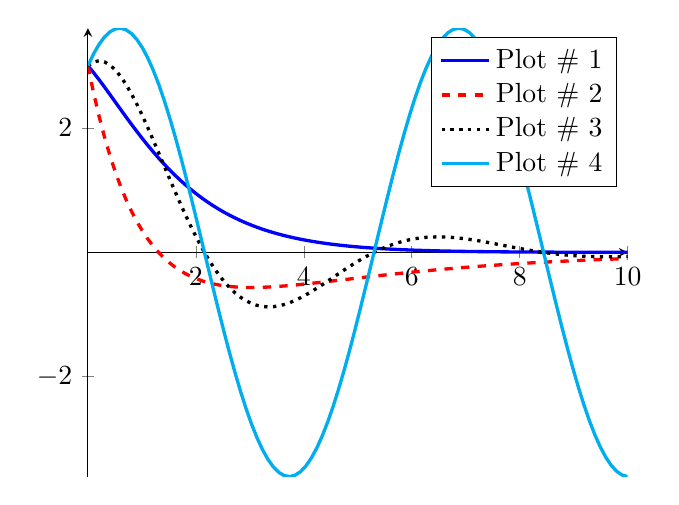
\begin{tikzpicture}
            \begin{axis}[axis lines=center, xmin=0, domain=0:10]
                \addplot[very thick, blue, samples=100] {3*exp(-x)+2*x*exp(-x)};
                \addlegendentry{Plot \# 1};
                \addplot[very thick, red, dashed, samples=100] {5*exp(-x)-2*exp(-0.3*x)};
                \addlegendentry{Plot \# 2};
                \addplot[very thick, black, dotted, samples=100] {exp(-0.4*x)*(2*sin(1*deg(x)) +
                3*cos(1*deg(x)))};
                \addlegendentry{Plot \# 3};
                \addplot[very thick, cyan, samples=100] {(2*sin(1*deg(x)) +
                3*cos(1*deg(x)))};
                \addlegendentry{Plot \# 4};
            \end{axis}
        \end{tikzpicture}
    \end{center}
\end{problem}
\solution{
Plot 1: critically damped, Plot 2: over damped, Plot 3: under damped
}

\begin{problem}
    A steel ball weighing 128 pounds is suspended from a spring.  This stretches the
    spring $\frac{128}{37}$ feet.  
    The ball is started in motion from the equilibrium position with a downward velocity
    of 5 feet per second (assume that the equilibrium position is $y=0$).  The air
    resistance (in pounds) of the moving ball numerically equals 4 times its velocity (in
    feet per second).  
    Suppose that after $t$ second the ball is $y$ feet below its rest position.  Find $y$
    in terms of $t$.  \\
    Note: The positive direction for $y$ is down and we can take as the gravitational acceleration 32 feet per second per second.
\end{problem}
\solution{
    If the ball pulls the spring by $\frac{128}{37}$ feet and is then at rest then we know
    from Newton's second law that 
    \[ mg = k \cdot \frac{128}{37} \]
    since the only acceleration acting on the ball is gravity.  The weight of the steel
    ball is 128 pounds which is equal to the gravitational force of the ball.  Hence, $mg
    = 128$ pounds.  Therefore 
    \[ 128 = k \cdot \frac{128}{37} \quad \implies \quad k = 37. \]

    From the other information in the problem we know that the differential equation
    modeling the motion is
    \[ 4 y'' + 4y' + 37 y = 0 \quad \text{with} \quad y(0) = 0 \text{ and } y'(0) = 5.
        \]
    The resulting characteristic polynomial is $4r^2 + 4r + 37 = 0$ and hence the roots
    are
    \[ r = \frac{-4 \pm \sqrt{16-4(4)(37)}}{8} = \frac{-4 \pm 24i}{8} =
    -\frac{1}{2} \pm 3i \]
    so the general solution to the differential equation is 
    \[ y(t) = e^{-(1/2)t} \left( C_1 \cos\left( 3t \right) + C_2
        \sin\left( 3 t \right) \right) \]
    Using the initial condition that $y(0) = 0$ we see that $C_1 = 0$ so the solution
    becomes
    \[ y(t) = Ce^{-(1/2)t} \sin\left( 3 t \right) \]
    The initial velocity is $y'(0) = 5$ so we next find the first derivative
    \[ y'(t) = -\frac{C}{2} e^{-(1/2)t} \sin(3t) + 3Ce^{-(1/2)t} \cos(3t) \]
    Using the initial velocity we get
    \[ 5 = 3C \quad \implies \quad C = \frac{5}{3}.  \]
    
    Therefore the solution is
    \[ y(t) = \frac{5}{3} e^{-(1/2)t} \sin(3t). \]


    \begin{center}
        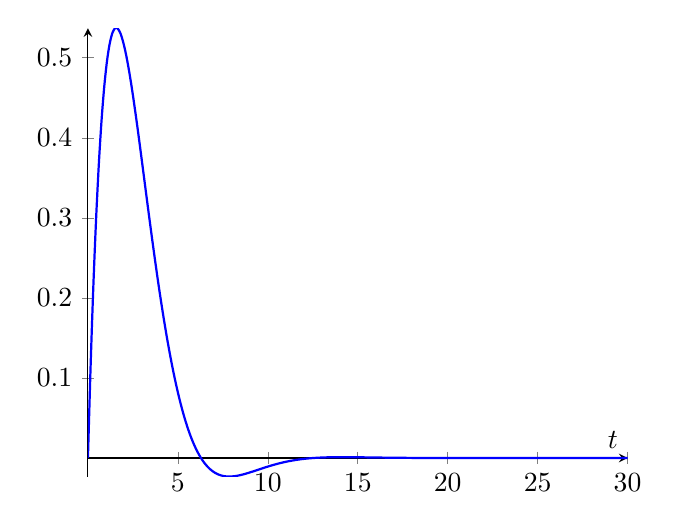
\begin{tikzpicture}
            \begin{axis}[axis lines=center, xmin=0, xmax=30, domain=0:30, xlabel={$t$}]
                \addplot[smooth, blue, thick, samples=200] {(5/3)*exp(-x/2)*sin(0.5*deg(x))};
            \end{axis}
        \end{tikzpicture}
    \end{center}
}



\section{Undetermined Coefficients}
In the previous section we were dealing with un-driven oscillators.  That is, the
oscillators had no external forces driving the oscillations aside from the initial
conditions.  In this section we'll consider what happens when you have an external driving
force.  From Newton's second law we can write the governing equation as
\begin{flalign}
    my'' + by' + ky = F_{external}
    \label{eqn:driven_oscillator}
\end{flalign}
where $F_{external}$ in \eqref{eqn:driven_oscillator} is a driving force beyond the
initial conditions, the spring constant, and the damping force.  

\begin{problem}
    Propose two different physical instances where an external driving force would
    influence the motion of an oscillator.
\end{problem}
\solution{
The presence of a magnetic field on an iron oscillator, a wind force blowing against the
oscillator, \ldots
}

\begin{problem}
    What is the equilibrium of the differential equation $4y''+5y'+y=1$?
\end{problem}
\solution{
If the motion stops then the $y''$ and $y'$ terms are zero and the equilibrium is $y=1$.
}

\begin{problem}
    Work with your partner(s) to suggest a solution technique for the non-homogenous
    linear second order differential equation $4y'' + 5y' + y = 1$.
\end{problem}
\solution{
    This problem can be solved by the method of undetermined coefficients. 
From Problem \ref{prob:classify_second_order} we know that the homogeneous solution is
\[ y_h(t) = C_1 e^{-(1/4)t} + C_2 e^{-t} \]
and since the non-homogeneity is constant we conjecture that 
\[ y_p(t) = C_3. \]
Therefore the general solution is
\[ y(t) = C_1 e^{-(1/4)t} + C_2 e^{-t} + C_3. \]
}



\begin{technique}
    To solve $my''+by'+ky=f(t)$:
    \begin{enumerate}
        \item Solve the homogeneous problem (taking $f(t)=0$)
        \item Find a particular solution to the non-homogeneous problem (same
            functional form as $f(t)$)
        \item IF the homogeneous and particular solutions are linearly independent
            then $y(t)$ is a linear combination of the homogeneous solutions and the
            particular solution
    \end{enumerate}
\end{technique}

Now let's put your undetermined coefficients skills to the test by solving the following
three un-damped driven oscillators.
\begin{problem}
    Solve $y''+4y = 2e^{3t}$ with $y(0)=0$  and $y'(0)=1$
\end{problem}
\solution{
    The natural frequency on the un-damped homogeneous oscillator is $\omega = \sqrt{4} =
    2$ so the homogeneous solution is $y_h(t) = C_1 \cos(2t) + C_2 \sin(2t)$.  The
    non-homogeneity is exponential so the particular solution is $y_p(t) = C_3 e^{3t}$
    making the general solution
    \[ y(t) = C_1 \cos(2t) + C_2 \sin(2t) + C_3 e^{3t}. \]
    Using the initial position we see that $0 = C_1 + C_3$.  To utilize the initial
    velocity we first observe that 
    \[ y'(t) = -2C_2 \sin(2t) + 2 C_2 \cos(2t) + 3 C_3 e^{3t}. \]
    From the initial velocity we see that $1=2C_2 + 3C_3$.

    To get the third equation necessary to find $C_1, C_2,$ and $C_3$ we substitute the
    particular solution into the differential equation to get
    \[ 9 C_3 e^{3t} + 4 C_3 e^{3t} = 2 e^{3t} \implies C_3 = \frac{2}{13}. \]
    Back substituting we find that $C_2 = 1 - 3C_3 = 1 - \frac{6}{13} =
    \frac{7}{13}$ and $C_1 = -\frac{2}{13}$.  Therefore the solution is
    \[ y(t) = -\frac{2}{13} \cos(2t) + \frac{7}{13}\sin(2t) + \frac{2}{13} e^{3t}. \]
}



\begin{problem}
    Solve $y''+4y = 5\sin(3t)$ with $y(0)=0$  and $y'(0)=1$
\end{problem}
\solution{
The natural frequency on the un-damped homogeneous oscillator is $\omega = \sqrt{4} =
    2$ so the homogeneous solution is $y_h(t) = C_1 \cos(2t) + C_2 \sin(2t)$.  The
    non-homogeneity is trigonometric with a different frequency as the natural frequency
    so $y_p(t) = C_3 \cos(3t) + C_4 \sin(3t)$ making the general solution
    \[ y(t) = C_1 \cos(2t) + C_2 \sin(2t) + C_3 \cos(3t) + C_4 \sin(3t). \]
    Using the initial position we see that $0 = C_1 + C_3$.  To utilize the initial
    velocity we first observe that 
    \[ y'(t) = -2C_1 \sin(2t) + 2C_2 \cos(2t) -3C_3 \sin(3t) + 3C_4 \cos(3t). \]
    From the initial velocity we see that $1 = 2C_2 + 3C_4$.

    The get the third and fourth equations necessary to find $C_1, C_2, C_3$ and $C_4$ we
    substitute the particular solution in to the differential equation to get
    \[ -9C_3\cos(3t) - 9C_4\sin(3t) + 4C_3\cos(3t) + 4C_4\sin(3t) = 5\sin(3t). \]
    Matching the coefficients of the cosine terms gives $-5 C_3 = 0$ and matching
    coefficients of the sine terms gives $-5 C_4 = 5$.  Hence, $C_3 = 0$ and $C_4 = -1$.  

    Back substituting gives $C_1 =0$ and $C_2 = 2.$  Hence the solution to the driven
    oscillator is
    \[ y(t) = 2 \sin(2t) - \sin(3t). \]
}

\begin{problem}
    Solve $y''+4y = 5\sin(2t)$ with $y(0)=0$  and $y'(0)=1$
\end{problem}
\solution{
We start again with a natural frequency of $\omega = 2$ but this time observe that the
driving frequency (on the right-hand side of the differential equation) exactly matches
the natural frequency of the homogeneous oscillator.  Therefore the homogeneous and
particular solutions will not be linearly independent  and the general solution is
\[ y(t) = C_1 \cos(2t) + C_2 \sin(2t) + C_3 t \cos(2t) + C_4 t \sin(2t). \]

From the initial position we know that $C_1 = 0$.  In order to utilize the initial
velocity we need $y'(t)$:
\begin{flalign*}
    y'(t) &= 2C_2 \cos(2t) + C_3 \left( -2t\sin(2t) + \cos(2t) \right) + C_4 \left( 2t\cos(2t)
    + \sin(2t) \right) \\
    &= 2C_2 \cos(2t) -2tC_3\sin(2t) + C_3\cos(2t) + 2tC_4 \cos(2t) + C_4\sin(2t) \\
    &= (2C_2 + C_3 + 2tC_4)\cos(2t) + (-2tC_3 + C4)\sin(2t).
\end{flalign*}
From the initial velocity we have $1 = 2C_2 + C_3$.

To find the next two equations we substitute the particular solution into the differential
equation to get
\begin{flalign*}
    & -4C_2\sin(2t) -2C_3\left( 2t\cos(2t) + \sin(2t) \right) -2C_3\sin(2t) +
    2C_4\left(-2t\sin(2t) +\cos(2t) \right) + 2C_4\cos(2t) \\
    &+ 4C_3 t \cos(2t) + 4C_4 t \sin(2t) = 5\sin(2t).
\end{flalign*}
Matching coefficients gives 
\begin{flalign*}
    -4C_2 -2C_3 - 2C_3 &= 5 \quad \text{(matching the $\sin(2t)$ coeffiecients)} \\
    2C_4 + 2C_4 &= 0 \quad \text{(matching the $\cos(2t)$ coeffiecients)}
\end{flalign*}
Putting the three equations together gives the system of equation
\[ \begin{pmatrix} 2 & 1 & 0 \\ -4 & -4 & 0 \\ 0 & 0 & 4 \end{pmatrix} \begin{pmatrix} C_2
        \\ C_3 \\ C_4 \end{pmatrix} = \begin{pmatrix} 1 \\ 5 \\ 0\end{pmatrix} \]
Clearly $C_4 = 0$ so we can reduce the system to
\[ \begin{pmatrix} 2 & 1  \\ -4 & -4 \end{pmatrix} \begin{pmatrix} C_2
        \\ C_3  \end{pmatrix} = \begin{pmatrix} 1 \\ 5 \end{pmatrix} \implies
            \left( \begin{array}{cc|c} 2 & 1 & 1 \\ -4 & -4 & 5 \end{array} \right) \to
                \left( \begin{array}{cc|c} 1 & 1/2 & 1/2 \\ 0 & -2 & 7 \end{array} \right)
                    \to \left( \begin{array}{cc|c} 1 & 0 & 9/4 \\ 0 & 1 & -7/2 \end{array} \right) \]
Finally we arrive at the solution
\[ y(t) = \frac{9}{4} \sin(2t) - \frac{7}{2} t \cos(2t). \]
}

\section{Resonance and Beats}
A particular type of forcing term occurs when there is a forcing term that matches the
natural frequency of the ocscillor.  In an un-damped oscillator this looks like:
\[ y'' + \omega^2 y = A \cos\left( \omega t \right). \]
Notice that the natural frequency of the homogeneous differential equation is the same as
the forcing term.  
\begin{problem}
    What is the homogeneous solution to the above equation?
    \[ y_{hom} = \underline{\hspace{2in}} \]
    and since the particular solution has the same frequency they are not linearly
    independent of those of the homogeneous solutions.  Propose a particular solution:
    \[ y_{particular} = \underline{\hspace{2in}}. \]
    The term that you proposed is the root cause of {\it resonance}.
\end{problem}

\begin{problem}
    In the differential equation $y'' + \omega^2 y = A \cos(\omega t)$ the amplitudes of
    the waves will grow in time.  What function do the amplitudes follow?
\end{problem}
\solution{
The amplitudes grow linearly due to the linear function multiplying the trigonometric
terms.
}

\begin{problem}
    Solve the differential equation $y'' + 144y = 4 \cos(12t)$ with $y(0) = 0$ and
    $y'(0)=0$
\end{problem}
\solution{
    $y(t) = \frac{1}{6}t\sin(12t)$
}

\begin{example}
    Resonance was responsible for the collapse of the Broughton suspension bridge near
    Manchester, England in 1831. The collapse occurred when a column of soldiers marched
    in cadence over the bridge, setting up a periodic force of rather large amplitude. The
    frequency of the force was approximately equal to the natural frequency of the bridge.
    Thus, the bridge collapsed when large oscillations occurred. For this reason soldiers
    are ordered to break cadence whenever they cross a bridge.

    The Millennium Bridge, the first new bridge to span the Thames River in London in over
    100 years, is a modern example of how resonance can effect a bridge.
    This pedestrian bridge, which opened to the public in June 2000, was quickly closed
    after the bridge experienced high amplitude horizontal oscillations during periods of
    high traffic. Studies by designers found that the bridge experienced high amplitude
    horizontal oscillations in response to horizontal forcing at a rate of one cycle per
    second. Typically, people walk at a rate of two steps per second, so the time between
    two successive steps of the left foot is about one second. Thus, if people were to
    walk in cadence, they would could set up strong horizontal forcing that would place a
    destructive load on the bridge. The engineers did not envision this to be a problem
    since tourists do not generally march in time. However, a video of tourists crossing
    the bridge revealed the opposite. When the bridge began oscillating, people tended to
    walk in time in order to keep their balance.\\
    \href{https://www.youtube.com/watch?v=gQK21572oSU}{https://www.youtube.com/watch?v=gQK21572oSU}
\end{example}
\solution{(Modified from \cite{Judson})
}

Now we consider what happens when the natural frequency of the homogeneous oscillator is
close but not exactly equal to that of the driving term.  First watch the video in the
example below.
\begin{example}
    For an example of the {\it beats} phenomenon see \\
    \href{https://www.youtube.com/watch?v=pRpN9uLiouI}{www.youtube.com/watch?v=pRpN9uLiouI}.
    This phenomenon occurs when the natural frequency and the forcing frequency differ by
    only a small amount.  
    \[ y'' + \omega_0^2 y = A \cos(\omega t) \]
    where $\omega_0$ and $\omega$ are very close but not the same.
    You will be playing with this in the lab.
\end{example}
\solution{(Modified from \cite{Judson})
}

\begin{problem}
    Go to the GeoGebra applet:
    \href{https://www.geogebra.org/m/T9yws7CB}{https://www.geogebra.org/m/T9yws7CB} and
    explore what happens to the sum of the two functions $f(x) = \sin(Ax)$ and $g(x) =
    \sin(Bx)$ when $A$ and $B$ are arbitrarily close to each other.
\end{problem}

\begin{problem}
    Use what you know about the previous problem to sketch the graphical solution to the
    differential equation $y'' + 4y = \sin(1.9t)$ with $y(0) = y'(0) = 0$.
\end{problem}

\begin{problem}
    Now solve the differential equation $y''+4y = \sin(1.9t)$ with $y(0) = y'(0) = 0$.
\end{problem}


To end this chapter we consider one more problem related to all of the differential
equations that you should know at this point.  
\begin{problem}
    Match the differential equations below to the solution plots further below.  There
    should be no need to actually solve the differential equations, but I won't stop you
    if that is what you really want to do. (there are 9 plots and 8 differential
    equations.  One plot does not have a match \dots just to keep you on your toes)
\begin{center}
    \begin{tabular}{|c|c|c|}
        \hline
        Differential Equation & Initial Conditions & Matches to Plot \# \\ \hline \hline
        $y'=0.2y(5-y)$ & $y(0)=1$ &  \\ \hline
        $y'' + y' + 25y = 0$ & $y(0)=0$ and $y'(0)=5$ &  \\ \hline
        $y''+25y=4\sin(5.5t)$ & $y(0)=0$ and $y'(0)=5$ &  \\ \hline
        $y'=-2y+10$ & $y(0)=1$ &  \\ \hline
        $y''+25y=4\sin(5t)$ & $y(0)=0$ and $y'(0)=5$ &  \\ \hline
        $y''+25y=0$ & $y(0)=0$ and $y'(0)=5$ &  \\ \hline
        $y'-0.2y=0$ & $y(0)=1$ &  \\ \hline
        $y'+0.2t=0$ & $y(0)=1$ &  \\ \hline
    \end{tabular}
\end{center}
\solution{8,6,4,3,1,2,7,9}
\def\scl{0.6}
\begin{center}
    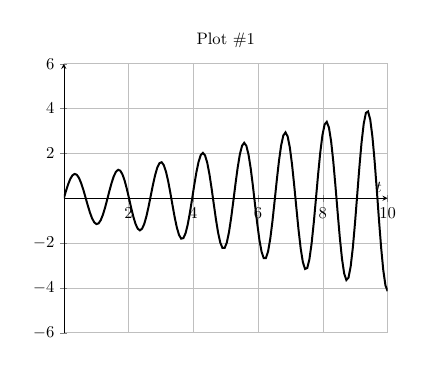
\begin{tikzpicture}[scale=\scl]
        \begin{axis}[axis lines=center, xlabel={$t$}, xmin=0, xmax=10, ymin=-6, ymax=6,
                grid, title={Plot \#1}]
                \addplot[very thick, domain=0:10, samples=150]
                {(1/25)*(-10*x*cos(deg(5*x)) + 26*sin(deg(5*x)) -
                cos(deg(10*x))*sin(deg(5*x)) + cos(deg(5*x))*sin(deg(10*x)))};
        \end{axis}
    \end{tikzpicture}
    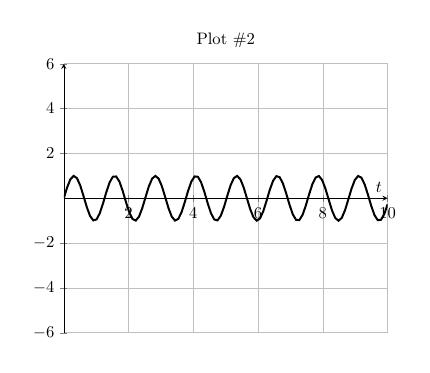
\begin{tikzpicture}[scale=\scl]
        \begin{axis}[axis lines=center, xlabel={$t$}, xmin=0, xmax=10, ymin=-6, ymax=6,
                grid, title={Plot \#2}]
                \addplot[very thick, domain=0:10, samples=100] {sin(deg(5*x))};
        \end{axis}
    \end{tikzpicture}
    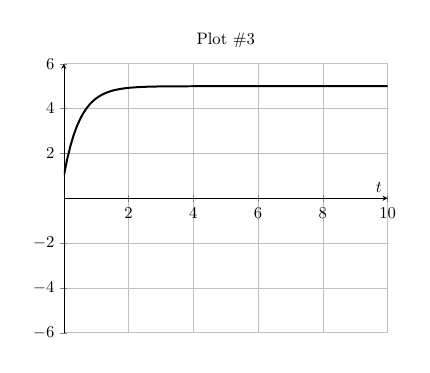
\begin{tikzpicture}[scale=\scl]
        \begin{axis}[axis lines=center, xlabel={$t$}, xmin=0, xmax=10, ymin=-6, ymax=6,
                grid, title={Plot \#3}]
                \addplot[very thick, domain=0:10, samples=100] {-4*exp(-2*x)+5};
        \end{axis}
    \end{tikzpicture}
\end{center}

\begin{center}
    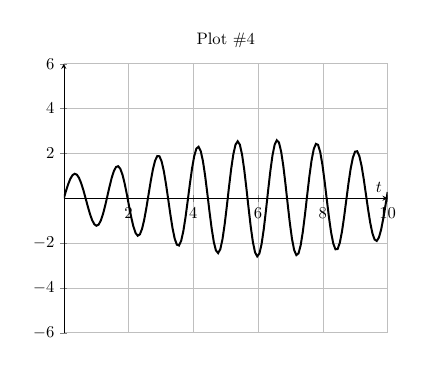
\begin{tikzpicture}[scale=\scl]
        \begin{axis}[axis lines=center, xlabel={$t$}, xmin=0, xmax=10, ymin=-6, ymax=6,
                grid, title={Plot \#4}]
                \addplot[very thick, domain=0:10, samples=150]
                {-0.8*(cos(deg(5*x))*sin(deg(0.5*x)) - 2.29762*sin(deg(5*x)) +
                cos(deg(0.5*x))*sin(deg(5*x)) + 0.047619*cos(deg(10.5*x))*sin(deg(5*x)) - 
              0.047619*cos(deg(5*x))*sin(deg(10.5*x)))};
        \end{axis}
    \end{tikzpicture}
    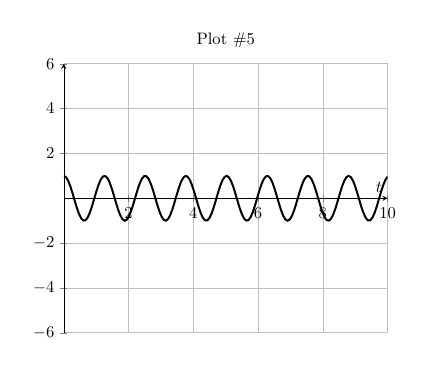
\begin{tikzpicture}[scale=\scl]
        \begin{axis}[axis lines=center, xlabel={$t$}, xmin=0, xmax=10, ymin=-6, ymax=6,
                grid, title={Plot \#5}]
                \addplot[very thick, domain=0:10, samples=150] {cos(deg(5*x))};
        \end{axis}
    \end{tikzpicture}
    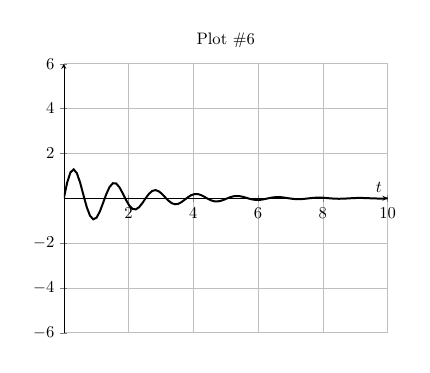
\begin{tikzpicture}[scale=\scl]
        \begin{axis}[axis lines=center, xlabel={$t$}, xmin=0, xmax=10, ymin=-6, ymax=6,
                grid, title={Plot \#6}]
                \addplot[very thick, domain=0:10, samples=100]
                {10/(2*sqrt(11))*exp(-x/2)*sin(deg(3*sqrt(11)*x/2))};
        \end{axis}
    \end{tikzpicture}
\end{center}
\begin{center}
    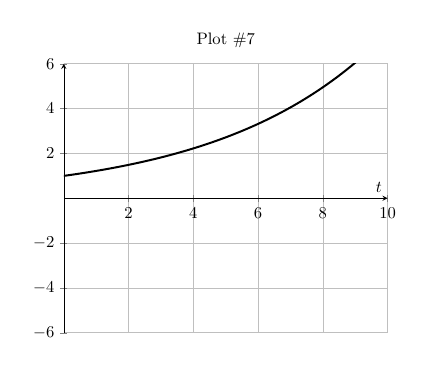
\begin{tikzpicture}[scale=\scl]
        \begin{axis}[axis lines=center, xlabel={$t$}, xmin=0, xmax=10, ymin=-6, ymax=6,
                grid, title={Plot \#7}]
                \addplot[very thick, domain=0:10, samples=100] {exp(0.2*x)};
        \end{axis}
    \end{tikzpicture}
    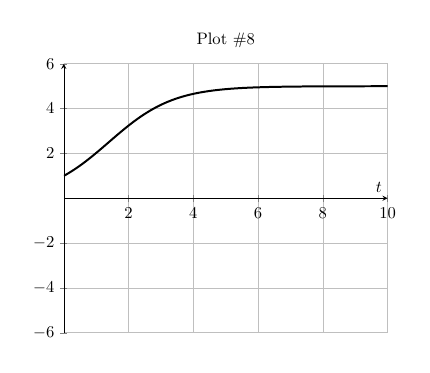
\begin{tikzpicture}[scale=\scl]
        \begin{axis}[axis lines=center, xlabel={$t$}, xmin=0, xmax=10, ymin=-6, ymax=6,
                grid, title={Plot \#8}]
                \addplot[very thick, domain=0:10, samples=150]
                {(5*exp(x))/(4+exp(x))};
        \end{axis}
    \end{tikzpicture}
    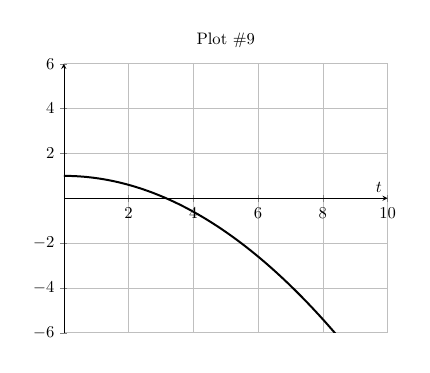
\begin{tikzpicture}[scale=\scl]
        \begin{axis}[axis lines=center, xlabel={$t$}, xmin=0, xmax=10, ymin=-6, ymax=6,
                grid, title={Plot \#9}]
                \addplot[very thick, domain=0:10, samples=100] {-0.1*x^2+1};
        \end{axis}
    \end{tikzpicture}
\end{center}
\end{problem}




\section{Additional Exercises}


\begin{problem}
\item Consider a floating cylindrical buoy with radius $r$, height $h$, and uniform
    density $\rho \le 0.5$ grams/cm$^3$.  The buoy is initially suspended at rest with
    its bottom at the top surface of the water and is released at $t=0$.  Thereafter
    it is acted on by two forces: 
    \begin{enumerate}
        \item a downward gravitational force equal to its weight: $mg = \left( \pi r^2 h
            \rho \right) g$, and
        \item an upward force due to buoyancy equal to the weight of the displaced water:
            $\left( \pi r^2 x\right) g$
    \end{enumerate}
    where $x$ is the depth of the bottom of the buoy beneath the surface at time $t$.
    (recall that the density of water is 1 gram/cm$^3$)
    \begin{itemize}
        \item[(a)] Write a differential equation modeling the depth of the buoy.
        \item[(b)] What type of motion does the buoy undergo?
        \item[(c)] What is the equilibrium of the oscillation?
        \item[(d)] What is the period of the oscillation?
    \end{itemize}
\end{problem}
\solution{
    \[ mx'' = \text{weight} - \text{buoyancy} \implies \rho \pi r^2 h x'' = \pi r^2 h
    \rho g - \pi r^2 g x \]
    \[ \implies x'' = g - \frac{g}{\rho h} x \implies x''=\frac{g}{\rho h} \left( \rho
        h - x
    \right) \]
    Substitute $y = \rho h -x$ so we see that $y''=-x''$ and we get
    \[ y'' + \frac{g}{\rho h} y = 0 \implies k^2 + \frac{g}{\rho h} = 0 \implies k =
    \pm \sqrt{\frac{g}{\rho h}} i \]
    \[ \implies y(t) = C_1 \cos\left( \sqrt{\frac{g}{\rho h}} t \right) + C_2 \sin
    \left( \sqrt{\frac{g}{\rho h}} t \right) \]
    \[ \implies x(t) = \rho h - \left[ C_1 \cos\left( \sqrt{\frac{g}{\rho h}} t \right) + C_2 \sin
    \left( \sqrt{\frac{g}{\rho h}} t \right) \right] \]

    Harmonic motion, period = $2\pi / \sqrt{g/(\rho h)} = 2\pi
    \sqrt{\frac{\rho h}{g}}$.  equilibrium = $\rho h$
}


\begin{problem}
    The previous problem does not account for the water's viscosity.  We can reframe the
    differential equation as 
    \[ mx'' = \text{weight} - \text{viscosity} - \text{buoyancy} \]
    and assume that the retarding force due to viscosity is proportional to the
    velocity of the buoy.
    \begin{itemize}
        \item[(a)] Write the resulting differential equation.
        \item[(b)] If $b$ represents the viscosity then what is the period of oscillation?
    \end{itemize}
\end{problem}
\solution{
    \[ \rho \pi r^2 h x'' = \pi r^2 h \rho g - b x' - \pi r^2 g x \implies x'' =
        \frac{g}{\rho h} \left( \rho h - x \right) - \frac{b}{\rho \pi r^2 h} x' 
    \]
    \[ \implies y'' + \frac{b}{\rho \pi r^2 h} y' + \frac{g}{\rho h} y = 0 \]
    \[ \implies k = \frac{-B \pm \sqrt{B^2 - 4 \frac{g}{\rho h}}}{2} =
        \frac{\frac{b}{\rho \pi r^2 h} \pm \sqrt{\frac{b^2}{\rho^2 \pi^2 r^4 h^2} -
    \frac{4g}{\rho h}   } }{2} \]
    \[ \implies \text{frequency} =\frac{1}{2} \sqrt{\frac{b^2}{\rho^2 \pi^2 r^4 h^2} -
    \frac{4g}{\rho h}} \]

}

